\section{Evaluation}
\label{sec:Experiments}

In this section, we would like to answer the following questions: (1) How do attention modules would affect the performance of grasp detection? What sort of attention modules is suitable for 3D point cloud data? How well do the learned models generalize to novel object categories? To answer the above questions, we conduct the experiments of grasp detection on the public dataset GraspNet-1Billion \cite{fang2020graspnet}. This is a large-scale grasp dataset collected from cluttered scenes considering multi-object-multi-grasp setting. The objects in GraspNet-1Billion have varying shapes, textures, sizes, materials, and underlying different occlusion conditions. Hence, it can be used to evaluate robustness to occlusion and the generalization ability of trained models.

%%%%%%%%%%%%%%%%%%%%%%%%%%%%%%%%%%%%%%%%%%%%%%%%%%%%%%%%%%%%%%%

\begin{figure*}[h!]
  \centering  
    \begin{subfigure}[b]{0.25\linewidth}
    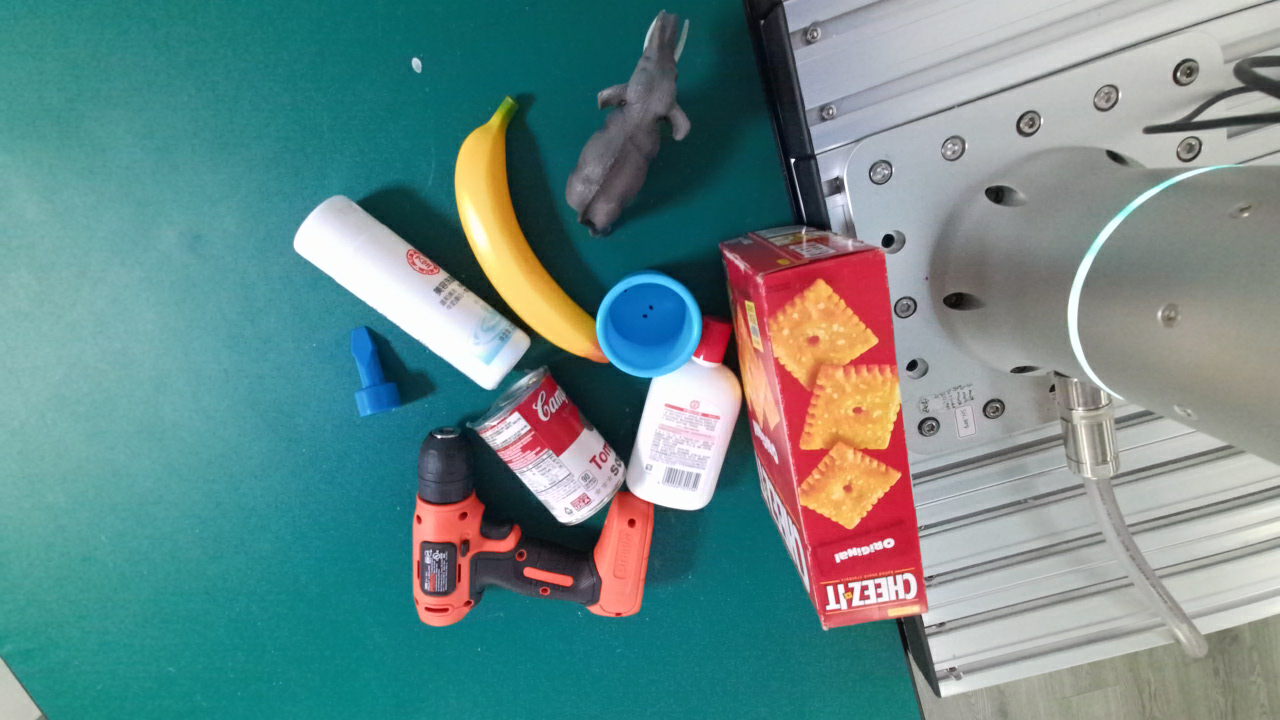
\includegraphics[width=5cm]{figs/Attention_module_results/color.png}
  \caption{}  
  \end{subfigure}
  
  %%%%%%%%%%%%%%%%%%%%%%%%%%%%%%%
  
  \begin{subfigure}[b]{0.32\linewidth}
    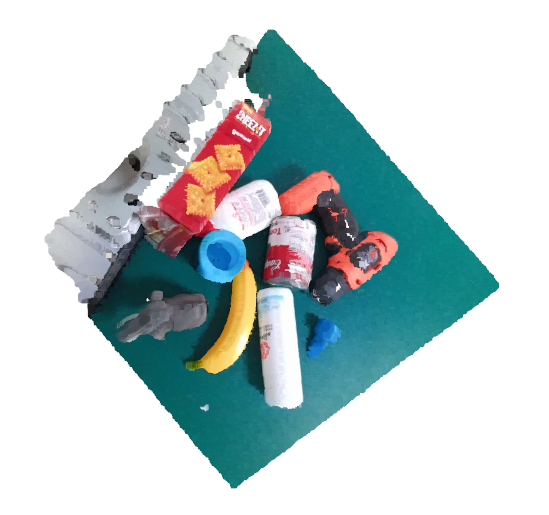
\includegraphics[width=5cm]{figs/Attention_module_results/pointcloud.png}
  \caption{}  
  \end{subfigure} 
  \begin{subfigure}[b]{0.32\linewidth}
    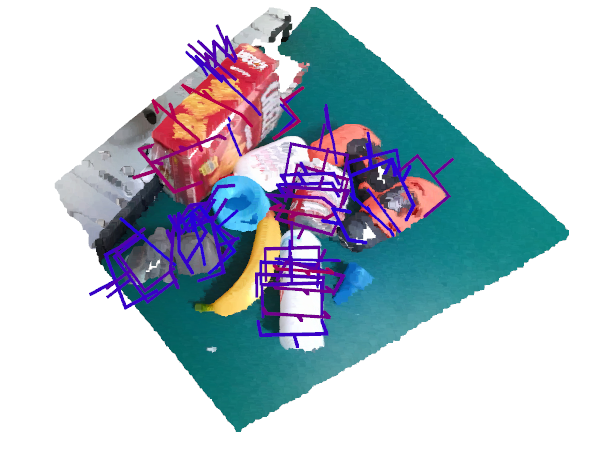
\includegraphics[width=5cm]{figs/Attention_module_results/Non-local.png}
    \caption{} 
  \end{subfigure} 
  \begin{subfigure}[b]{0.32\linewidth}
    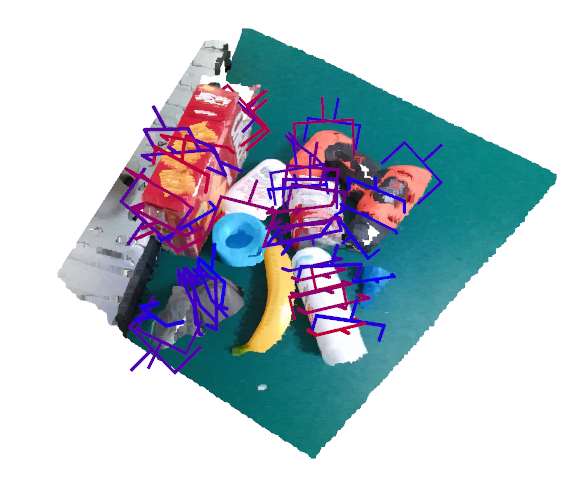
\includegraphics[width=5cm]{figs/Attention_module_results/Criss-cross.png}
  \caption{}  
  \end{subfigure}
  
  %%%%%%%%%%%%%%%%%%%%%%%%%%%%%%%%%%%%%%%%%%%%%%%%
  
    \begin{subfigure}[b]{0.32\linewidth}
    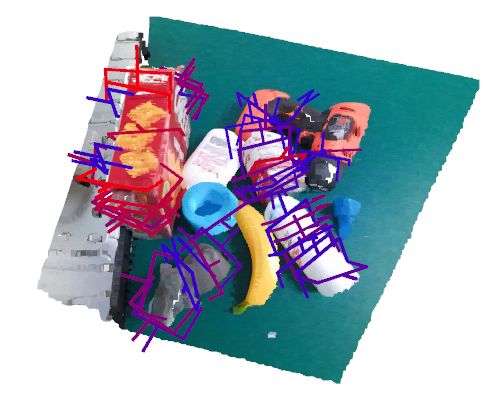
\includegraphics[width=5cm]{figs/Attention_module_results/SE.png}
  \caption{}  
  \end{subfigure}   
  \begin{subfigure}[b]{0.32\linewidth}
    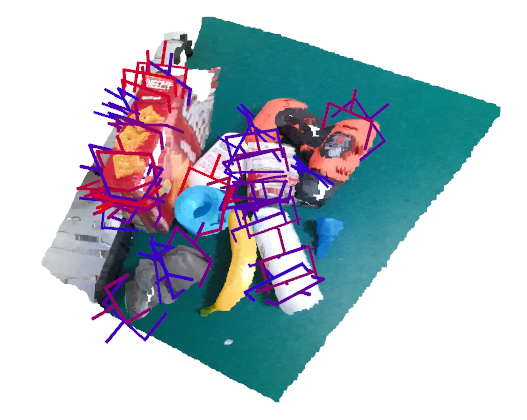
\includegraphics[width=5cm]{figs/Attention_module_results/CGNL.png}
    \caption{} 
  \end{subfigure}   
      \begin{subfigure}[b]{0.32\linewidth}
    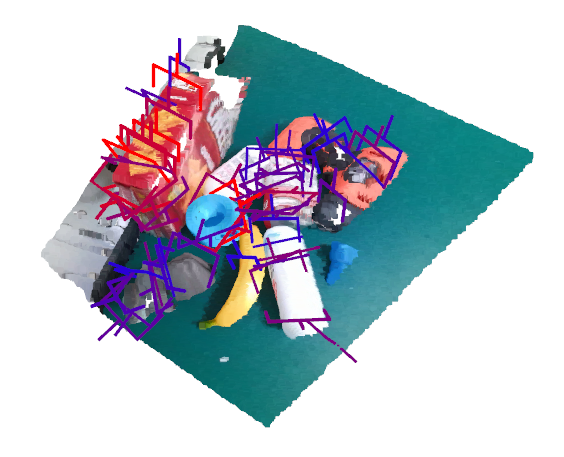
\includegraphics[width=5cm]{figs/Attention_module_results/DANet.png}
    \caption{} 
  \end{subfigure} 
  
   %%%%%%%%%%%%%%%%%%%%%%%%%%%%%%%%% 
   
    \begin{subfigure}[b]{0.25\linewidth}
    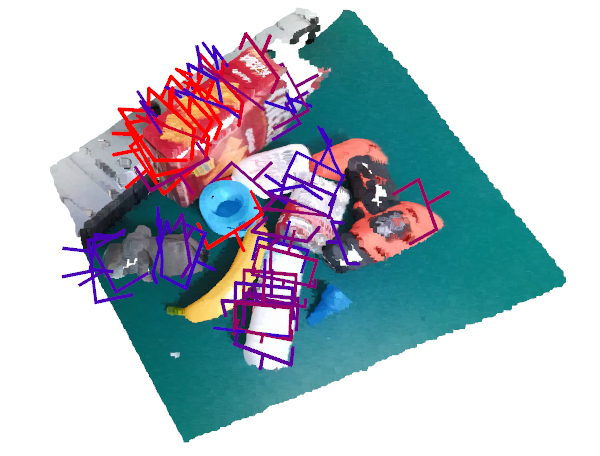
\includegraphics[width=5cm]{figs/Attention_module_results/CBAM.png}
    \caption{} 
  \end{subfigure} 
    \begin{subfigure}[b]{0.32\linewidth}
    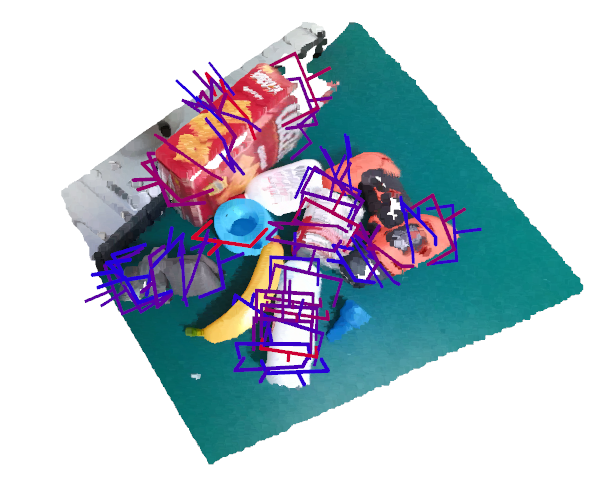
\includegraphics[width=5cm]{figs/Attention_module_results/Point-Attention.png}
    \caption{} 
  \end{subfigure} 
    \begin{subfigure}[b]{0.32\linewidth}
    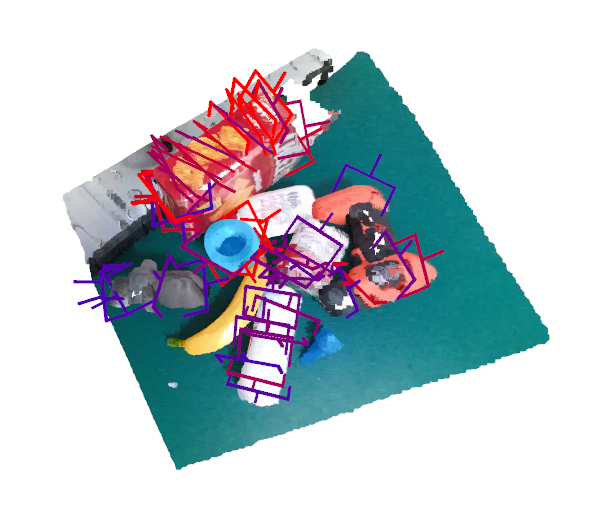
\includegraphics[width=5cm]{figs/Attention_module_results/Point_Transformer.png}
    \caption{} 
  \end{subfigure}
  
  \caption{Examples of input point clouds and predicted grasps from VoteGrasp combining with different attention module; (a) experiment objects; (b) input point cloud; (c) Non-local; (d) Criss-cross; (e) Squeeze-and-Excitation; (f) Compact Generalized Non-local; (g) Dual Attention Network; (h) Convolution Block Attention Module; (i) Point attention; (j) Point transformer. The different intensity of grasp color denotes the confident score of grasps. Red refers to the highest quality grasps and blue refers to the lowest ones.}
  \label{fig:grasp_pred_result}
\end{figure*}

%%%%%%%%%%%%%%%%%%%%%%%%%%%%%%%%%%%%%%%%%%%%%%%%%%%%%%%%%%%%%%%

\subsection{GraspNet-1Billion}

The GraspNet-1Billion (\textcolor{cyan}{\cite{fang2020graspnet}}) consists of 97,280 RGB-D images captured from 190 cluttered scenes. The dataset provides over one billion grasp poses for 88 objects presented in the scenes and an accurate 3D mesh model of each object is available as well. Besides, it also provides relevant information including camera poses, 6D object poses, object masks, and bounding boxes for all frames. The rich annotations allow us to generate ground truth votes and grasp configurations easily. Following (\textcolor{cyan}{\cite{fang2020graspnet}}) we split the dataset into 100 scenes for training and 90 scenes for testing. To evaluate model generalizability, the test sets are divided into 30 scenes with novel objects, 30 for unseen but similar objects, and the rest for seen objects.

\subsection{Implementation}

%%%%%%%%%%%%%%%%%%%%%%%%%%%%%%%%%%%%%%%%%%%%%%%%%%%%%%%%%%%

\begin{table}[h]
\caption{Layer parameters of the PointNet++ (\textcolor{cyan}{\cite{qi2017pointnet++}}) based feature learning network.}
\label{tab:layer_specs}
\begin{center}
\begin{tabular}{|l|c|c|}
\hline
layer name & input layer & layer params \\
\hline
SA1 & point cloud & (2048,0.025,[64,64,128]) \\
SA2 & SA1  & (1024,0.05,[128,128,256]) \\
SA3 & SA2 & (512,0.1,[128,128,256]) \\
SA4 & SA3 & (256,0.2,[128,128,256]) \\
FP1 & SA3, SA4 & [256,256] \\ 
FP2 & SA2, SA3 & [256,256] \\
\hline
\end{tabular}
\end{center}
\end{table}
%%%%%%%%%%%%%%%%%%%%%%%%%%%%%%%%%%%%%%%%%%%%%%%%%%%%%%%%%%%

In our implementation\footnote{Our code and other materials are available at \url{https://github.com/hoangcuongbk80/NovelVoteGrasp}}, we randomly choose $N$=50k points from each raw point cloud. We then apply the PointNet++ (\textcolor{cyan}{\cite{qi2017pointnet++}}) based feature learning network, which has 4 set abstraction layers (SA) and 2 feature propagation layers (FP). The detailed layer parameters are shown in Table~\ref{tab:layer_specs}. The FP2 outputs $M=1024$ seeds with $F=256-dim$ features and 3D coordinates that will be transformed to votes. The voting module generates $J=10$ votes per seed with an MLP layer spec: $[256, 256, 259 \times 10]$. In the attention module, we form $K=1024$ clusters and output a new feature map $C_{context} \in K \times F'$ where $K=1024, F'=128$. In the last step, 1024 grasps are detected from the new feature map. The prediction layer has $5 + V + 2A$ channels where $V=120$, and $A=6$.

The implementations are realized by PyTorch and Python platforms on one Nvidia GeForce RTX 2080 Ti 10GB GPU using CUDA and Linux operating system. All the experiments adopt similar training settings. The networks are trained from scratch in an end-to-end manner. We train each model over 200 epochs with stochastic gradient descent using a batch size of 8 and the Adam optimizer with a learning rate of 0.001.

\subsection{Metrics}

To evaluate the performance of grasp detection, we follow prior work (\textcolor{cyan}{\cite{fang2020graspnet}}) and report results using $Precision@k$. This metric measures the precision of top-k ranked grasps. We first check whether a predicted grasp ($G_{p}$) is true positive or not. It is considered a true positive only if the grasp satisfies three conditions: (i) there is an object inside the gripper; (ii) it is collision-free; (iii) the grasp is antipodal under a given friction coefficient $\mu$. The third condition is computed based on the prior works (\textcolor{cyan}{\cite{ten2017grasp, fang2020graspnet}}). We let $AP_{\mu}$ denote the average $Precision@k$ for $k$ ranges from 1 to 50 given a friction coefficient $\mu$. We report the average of $AP_{\mu}$ with $\mu = \left\lbrace 0.2,0.4,0.6,0.8,1.0 \right\rbrace $, denoted as \textbf{AP}.

\subsection{Results}

%%%%%%%%%%%%%%%%%%%%%%%%%%%%%%%%%%%%%%%%%%%%%%%%%%%%%%%%%%%
\begin{table}[h]
\caption{Inference Time of VoteGrasp with different attention modules, evaluated on GraspNet-1Billion (\textcolor{cyan}{\cite{fang2020graspnet}}) dataset.}
\label{tab:real_ex}
\begin{center}
\begin{tabular}{|l|c|c|}
\hline
Method & Inference Time (ms) \\
\hline
Non-local & 140 \\
\hline
CGNL & 150 \\
\hline
Criss-cross & 138 \\
\hline
Squeeze-and-Excitation (SE) & 135 \\
\hline
CBAM & 143 \\
\hline
DANet & 145 \\
\hline
Point Transformer & 170 \\
\hline
Point-Attention & 148 \\
\hline
\end{tabular}
\end{center}
\end{table}
%%%%%%%%%%%%%%%%%%%%%%%%%%%%%%%%%%%%%%%%%%%%%%%%%%%%%%%%%%%

%%%%%%%%%%%%%%%%%%%%%%%%%%%%%%%%%%%%%%%%%%%%%%%%%%%%%%%%%%%

\begin{table*}[h]
\caption{The table shows the results on GraspNet-1Billion test set captured by RealSense sensor.}
\label{tab:grasp_detect_eval_RealSense}
\begin{center}
\begin{tabular}{|l|c|c|c|c|c|c|c|c|c|}
\hline
& \multicolumn{3}{c|}{Seen} & \multicolumn{3}{c|}{Unseen (but similar)} & \multicolumn{3}{c|}{Novel} \\
\hline
& $AP$ & $AP_{0.8}$ & $AP_{0.4}$ & $AP$ & $AP_{0.8}$ & $AP_{0.4}$ & $AP$ & $AP_{0.8}$ & $AP_{0.4}$  \\
\hline
\textbf{Non-local} & 28.06 & 32.24 & 18.43 & 26.30 & 35.29 & 14.92 & 11.79 & 11.83 & 6.62 \\
\hline
\textbf{Criss-cross} & 29.01 & 33.37 & 18.84 & 27.44 & 36.62 & 15.72 & 12.26 & 12.43 & 6.77 \\
\hline
\textbf{Squeeze-and-Excitation (SE)} & 32.18 & 37.32 & 22.01 & 30.60 & 39.73 & 18.98 & 15.91 & 16.06 & 8.05 \\
\hline
\textbf{CGNL} & 34.13 & 38.87 & 24.04 & 33.03 & 40.78 & 20.54 & 16.92 & 17.03 & 10.01 \\
\hline
\textbf{CBAM} & 36.70 & 41.08 & 27.04 & 35.23 & 43.62 & 22.83 & 21.08 & 20.69 & 10.25 \\
\hline
\textbf{DANet} & 34.02 & 38.51 & 24.00 & 32.87 & 40.01 & 20.12 & 16.50 & 17.00 & 9.83 \\
\hline
\textbf{Point Transformer} & \textbf{41.45} & \textbf{45.63} & \textbf{32.42} & \textbf{40.12} & \textbf{48.40} & \textbf{27.21} & \textbf{26.02} & \textbf{26.23} & \textbf{14.18} \\
\hline
\textbf{Point-Attention} & 26.34 & 30.40 & 17.18 & 24.26 & 33.35 & 12.72 & 10.68 & 10.82 & 6.05 \\
\hline

\end{tabular}
\end{center}
\end{table*}
%%%%%%%%%%%%%%%%%%%%%%%%%%%%%%%%%%%%%%%%%%%%%%%%%%%%%%%%%%%

%%%%%%%%%%%%%%%%%%%%%%%%%%%%%%%%%%%%%%%%%%%%%%%%%%%%%%%%%%%

\begin{table*}[h]
\caption{The table shows the results on GraspNet-1Billion test set captured by Kinect sensors respectively.}
\label{tab:grasp_detect_eval_Kinect}
\begin{center}
\begin{tabular}{|l|c|c|c|c|c|c|c|c|c|}
\hline
& \multicolumn{3}{c|}{Seen} & \multicolumn{3}{c|}{Unseen (but similar)} & \multicolumn{3}{c|}{Novel} \\
\hline
& $AP$ & $AP_{0.8}$ & $AP_{0.4}$ & $AP$ & $AP_{0.8}$ & $AP_{0.4}$ & $AP$ & $AP_{0.8}$ & $AP_{0.4}$  \\
\hline
Non-local & 31.52 & 40.37 & 21.19 & 30.57 & 38.40 & 18.67 & 13.05 & 13.19 & 7.03 \\
\hline
Criss-cross & 32.29 & 40.85 & 21.91 & 31.23 & 39.07 & 19.09 & 13.82 & 13.93 & 7.08 \\
\hline
Squeeze-and-Excitation (SE) & 35.93 & 43.85 & 24.05 & 33.68 & 41.09 & 21.58 & 16.00 & 16.09 & 8.29 \\
\hline
CGNL & 37.52 & 45.61 & 27.68 & 35.86 & 43.31 & 24.74 & 18.46 & 18.49 & 10.63 \\
\hline
CBAM & 39.98 & 48.60 & 28.79 & 38.24 & 46.02 & 26.25 & 21.30 & 20.59 & 10.34 \\
\hline
DANet & 37.36 & 45.17 & 27.32 & 35.38 & 43.02 & 24.15 & 18.02 & 18.09 & 10.23 \\
\hline
Point Transformer & \textbf{44.80} & \textbf{52.47} & \textbf{33.03} & \textbf{42.19} & \textbf{50.18} & \textbf{30.58} & \textbf{26.21} & \textbf{26.69} & \textbf{14.50} \\
\hline
Point-Attention & 29.01 & 37.62 & 19.19 & 27.63 & 36.21 & 16.32 & 11.35 & 11.68 & 6.80 \\
\hline
\end{tabular}
\end{center}
\end{table*}
%%%%%%%%%%%%%%%%%%%%%%%%%%%%%%%%%%%%%%%%%%%%%%%%%%%%%%%%%%%

We examine VoteGrasp with different self-attention modules in GraspNet-1Billion dataset captured by RealSense sensor and Kinect sensor and the results are shown in Table. \ref{tab:grasp_detect_eval_RealSense} and Table. \ref{tab:grasp_detect_eval_Kinect} respectively. Two tables witness a similar trend of grasp precision of attention modules in testing with seen, unseen (but similar), and novel objects. Point attention module yields severest grasp detection accuracy in all practicing conditions. Non-local and Criss-cross networks both using only position attention gain approximate accuracy and are slightly higher than point attention. Whereas, SE instead focuses on channel correlations and meets more reliable grasps than solely employing positional distribution. CGNL fusing information of pixels' position into feature vectors obtains better grasp detection. Leveraging both position attention module and channel attention module, CBAM and DANet acquire significant grasp accuracy than the previously mentioned blocks. However, arranging two attention modules in sequence as CBAM achieves marginally reasonable grasps than placing them in parallel as DANet. Finally, point transformer outperforms all others with huge significance of grasp accuracy at $41.63\%$ averaged AP from both cameras. Besides, we investigate inference time of VoteGrasp with different attention modules. We perceive that all versions consume approximate time around $135ms$ to $170ms$ as shown in Table. \ref{tab:real_ex}. Point transformer, which achieves best result of grasp detection, takes $170ms$. Therefore, this block is considered as the preferred solution to be combined with VoteGrasp to achieve optimal robustness. 

\section{Conclusions}

In this work, we conduct VoteGrasp with a set of attention modules. Thereby, we provide insights about attention mechanism and its ability to be integrated with grasp detection architecture as well. Taking advantage of VoteGrasp in grasp detection, we examine the performance of different attention modules to discover the optimal combination for collision-free grasps. Through experiments, we verify that point transformer is the ideal choice to achieve high-quality grasps in occlusions and cluttered scenes. This attention module guarantees VoteGrasp's ability to generalize to highly occluded objects and even novel objects while keeping the model to be lightweight. Interesting future work is to consider adding a reachability predictor to the grasping network and explore the use of our approach in task planning applications.
